\documentclass[11pt]{article}
% generated by Madoko, version 1.2.3
%mdk-data-line={1}


\usepackage[heading-base={2},section-num={False},bib-label={hide},fontspec={True}]{madoko2}
\usepackage[top=1in, bottom=1.25in, left=1in, right=1in]{geometry}
\usepackage{fancyhdr}
\usepackage{mathpartir}
%mdk-data-line={13}

  \setlength{\headheight}{30pt}
  \renewcommand{\footrulewidth}{0.5pt}

\begin{document}



{\mdfontfamily{UtopiaStd-Regular}
%mdk-data-line={140}
\mdxtitleblockstart{}
%mdk-data-line={140}
\mdxtitle{{\sffamily{\bfseries\mdline{140}Petr4 Type System Formalization}}}%mdk
\mdxauthorstart{}
%mdk-data-line={145}
\mdxauthorname{\mdline{145}Parisa Ataei, Ryan Doenges, Nate Foster}%mdk

%mdk-data-line={148}
\mdxauthoraddress{\mdline{148}Cornell University}%mdk
\mdxauthorend
%mdk-data-line={155;ops.tex:3}
\mdxtitlefooter{{\sffamily{\bfseries\mdline{155;ops.tex:3}2022-05-11}}}%mdk
\mdtitleauthorrunning{}{}\mdxtitleblockend%mdk

%mdk-data-line={142}
\begin{abstract}%mdk

%mdk-data-line={143}
\noindent\mdline{143}P4 is a language for programming the data plane of network
devices. Petr4 provides a clean-slate definitional interpreter
and a core calculus that models a fragment of P4. This document
provides a definition of Petr4\mdline{146}'\mdline{146}s type system that is consistent
with its implementation. The target audience of this document
includes developers and debuggers who work on P4 implementations
such as Petr4 and P4C. In essence, this document may be of
interest to programmers who are interested in understanding
the implementation of Petr4 deeply.%mdk
%mdk
\end{abstract}%mdk
%mdk-data-line={155;ops.tex:1}
%stuff here and there:
\renewcommand{\or}{\ | \ }
\newcommand{\whereBulletIs}{,\textit{ where } \bullet \textit{ is }}
\newcommand{\whereIs}[1]{,\textit{ where } {#1} \textit{ is }}
\newcommand{\where}[1]{,\textit{ where } {#1}}
\newcommand{\textOr}{\textit{ or }}
\newcommand{\numeric}[1]{\mathit{numeric}({#1})}
\newcommand{\error}{\mathit{error}}
\newcommand{\cond}{\mathit{cond}}
\newcommand{\prim}[1]{{#1}^\prime}
\newcommand{\pprim}[1]{{#1}^{\prime\prime}}

%typing judgments:
\newcommand{\envOne}[2]{\Delta, T, \Gamma \vdash {#1} : {#2}}
\newcommand{\expenv}[4]{\env, \ctxt \vdash {#1} \leadsto {#2}, {#3}, {#4}}
\newcommand{\expenvWithCtxt}[5]{\env, {#1} \vdash {#1} \leadsto {#2}, {#3}, {#4}}
\newcommand{\coerceBinArgsEnv}[3]{\env, \ctxt \vdash {#1} \twoheadrightarrow {#2} {#3}}
\newcommand{\binOpEnv}[4]{\env \vdash {#1} \hookrightarrow {#2} {#3} {#4}}

%contexts:
\newcommand{\cte}{\mathit{CONSTANT}}

%metavariables:
\newcommand{\env}{e}
\newcommand{\typ}{t}
\newcommand{\ctxt}{c}
\newcommand{\bool}{b}
\newcommand{\str}{s}
\newcommand{\width}{w}
\newcommand{\val}{v}
\newcommand{\bit}{\mathit{bit}}
\renewcommand{\int}{n}
\newcommand{\bitWidth}[2]{{#1}_{#2}}
\newcommand{\intWidth}[2]{{#1}_{#2}}
\newcommand{\name}{\mathit{name}}
\renewcommand{\array}{a}
\renewcommand{\index}{i}
\newcommand{\arrayAccess}[2]{{#1}[{#2}]}
\newcommand{\size}{n}
\newcommand{\high}{h}
\newcommand{\low}{l}
\newcommand{\bitString}{bs}
\newcommand{\bitStringAccess}[3]{{#1}[{#2}:{#3}]}
\renewcommand{\exp}{\mathit{exp}}
\newcommand{\field}{f}

%function helpers
\newcommand{\isNumeric}[1]{\mathit{is\_numeric}({#1})}
\newcommand{\isArray}[1]{\mathit{is\_array}({#1})}
\newcommand{\compileTimeEval}[1]{[[{#1}]]_\env}

%types:
\newcommand{\bitWidthTyp}[1]{\mathit{bit}<\!{#1}\!>}
\newcommand{\intWidthTyp}[1]{\mathit{int}<\!{#1}\!>}
\newcommand{\boolTyp}{\mathit{bool}}
\newcommand{\stringTyp}{\mathit{string}}
\newcommand{\integerTyp}{\mathit{integer}}
\newcommand{\bitStringTyp}[2]{\mathit{bit[{#1}-{#2}]}}
\newcommand{\intTyp}{\mathit{int}}

%directions:
\newcommand{\less}{\mathit{directionless}}
\newcommand{\dir}{d}
\renewcommand{\in}{\mathit{in}}
\newcommand{\out}{\mathit{out}}

\mdline{158}
\begin{mdtoc}%mdk

\section*{Contents}\mdlabel{sec-contents}{2}%mdk%mdk

\begin{mdtocblock}%mdk

\mdtocitemx{sec-overview}{\mdref{sec-overview}{1.\hspace*{0.5em}Overview}}%mdk

\begin{mdtocblock}%mdk

\mdtocitemx{sec-conn}{\mdref{sec-conn}{1.1.\hspace*{0.5em}Connecting To The Implementation}}%mdk

\mdtocitemx{sec-arch}{\mdref{sec-arch}{1.2.\hspace*{0.5em}Architecture}}%mdk
%mdk
\end{mdtocblock}%mdk

\mdtocitemx{sec-type-system}{\mdref{sec-type-system}{2.\hspace*{0.5em}Type System}}%mdk

\begin{mdtocblock}%mdk

\mdtocitemx{sec-expressions-typing-rules}{\mdref{sec-expressions-typing-rules}{2.1.\hspace*{0.5em}Expression's Typing Rules}}%mdk

\begin{mdtocblock}%mdk

\mdtocitemx{sec-coerce-binary-operation-arguments-helper}{\mdref{sec-coerce-binary-operation-arguments-helper}{2.1.1.\hspace*{0.5em}Coerce Binary Operation Arguments Helper}}%mdk

\mdtocitemx{sec-check-binary-operation-helper}{\mdref{sec-check-binary-operation-helper}{2.1.2.\hspace*{0.5em}Check Binary Operation Helper}}%mdk
%mdk
\end{mdtocblock}%mdk
%mdk
\end{mdtocblock}%mdk
%mdk
\end{mdtocblock}%mdk
%mdk
\end{mdtoc}%mdk

%mdk-data-line={160}
\section{\mdline{160}1.\hspace*{0.5em}\mdline{160}Overview}\mdlabel{sec-overview}{1}%mdk%mdk

%mdk-data-line={162}
\noindent\mdline{162}This document defines the type system of Petr4. The type system
conducts three tasks simultaneously:%mdk

%mdk-data-line={165}
\begin{enumerate}[noitemsep,topsep=\mdcompacttopsep]%mdk

%mdk-data-line={165}
\item\mdline{165}It type checks P4 programs.%mdk

%mdk-data-line={166}
\item\mdline{166}It conducts type inference.%mdk

%mdk-data-line={167}
\item\mdline{167}It does a pass from the surface syntax to the first IR.%mdk
%mdk
\end{enumerate}%mdk

%mdk-data-line={170}
\subsection{\mdline{170}1.1.\hspace*{0.5em}\mdline{170}Connecting To The Implementation}\mdlabel{sec-conn}{1.1}%mdk%mdk

%mdk-data-line={172}
\noindent\mdline{172}The following locates each data type in the implementation
(\mdline{173}\href{https://github.com/verified-network-toolchain/petr4}{{\ttfamily https://\hspace{0pt}github.\hspace{0pt}com/\hspace{0pt}verified-\hspace{0pt}network-\hspace{0pt}toolchain/\hspace{0pt}petr4}}\mdline{173}):%mdk

%mdk-data-line={175}
\begin{itemize}[noitemsep,topsep=\mdcompacttopsep]%mdk

%mdk-data-line={175}
\item\mdline{175}The surface AST is \mdline{175}\emph{types.program}\mdline{175}%mdk

%mdk-data-line={176}
\item\mdline{176}The type of programs of the surface syntax is \mdline{176}\emph{types.type.t}\mdline{176}%mdk

%mdk-data-line={177}
\item\mdline{177}The first IR is \mdline{177}\emph{prog.program}\mdline{177}%mdk

%mdk-data-line={178}
\item\mdline{178}The type of the first IR is \mdline{178}\emph{prog.type.t}\mdline{178}%mdk
%mdk
\end{itemize}%mdk

%mdk-data-line={180}
\noindent\mdline{180}For simplicity, we have removed the information that is needed to report when an error
happens. Such information is passed around in the surface syntax as a field (called
\mdline{182}\mdcode{{\mdfontfamily{LuxiMono}{\mdfontsize{\dimfont{0.75}}tags}}}\mdline{182}) of record for all data types.%mdk

%mdk-data-line={184}
\subsection{\mdline{184}1.2.\hspace*{0.5em}\mdline{184}Architecture}\mdlabel{sec-arch}{1.2}%mdk%mdk

%mdk-data-line={186}
\noindent\mdline{186}Figure\mdline{186}~\mdref{fig-arch}{\mdcaptionlabel{1}}\mdline{186} depicts part of Petr4\mdline{186}'\mdline{186}s architecture that contains the type system.
After lexing and parsing a P4 program we get a program in our surface syntax. This
program is then passed through the \mdline{188}\emph{elaborator}\mdline{188} where type variables are introduced
instead of underscore and new type variable names are generated for variables with the
same name but in different scopes. This document does not discuss the innerworkings of
\mdline{191}\mdcode{{\mdfontfamily{LuxiMono}{\mdfontsize{\dimfont{0.75}}elaborate}}}\mdline{191}. Then, the program is passed through the type system (encoded in \mdline{191}\mdcode{{\mdfontfamily{LuxiMono}{\mdfontsize{\dimfont{0.75}}checker}}}\mdline{191}).
This document discusses the innerworking of the type system extensively. Finally, the
program is evaluated.%mdk

%mdk-data-line={195}
\begin{figure}[tbp]%mdk
\begin{mdcenter}%mdk

%mdk-data-line={196}
\noindent\mdline{196}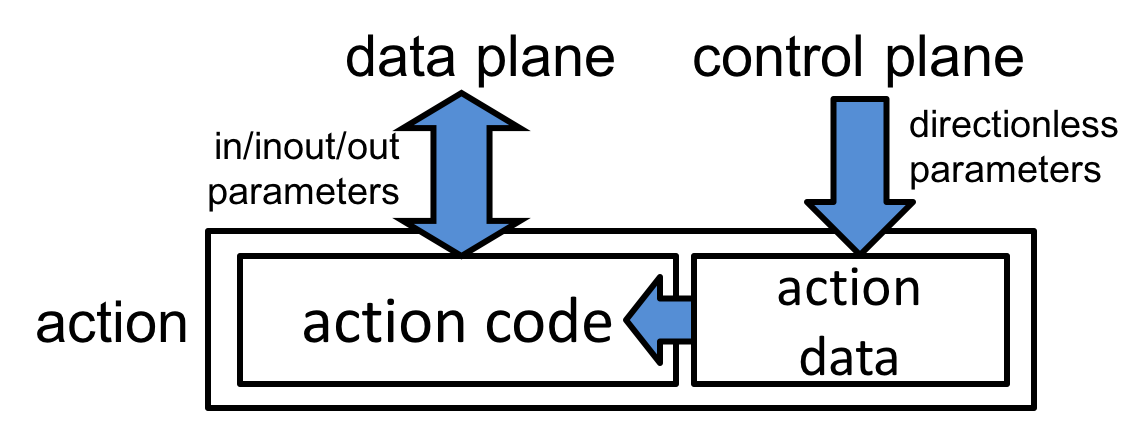
\includegraphics[keepaspectratio=true,width=\dimwidth{1.00}]{figs/petr4/arch}{}\mdline{196}%mdk

%mdk-data-line={197}
\mdhr{}%mdk

%mdk-data-line={198}
\noindent\mdline{198}\mdcaption{\textbf{Figure~\mdcaptionlabel{1}.}~\mdcaptiontext{Part of Petr4's achitecture.}}%mdk
%mdk
\end{mdcenter}\mdlabel{fig-arch}{1}%mdk
%mdk
\end{figure}%mdk

%mdk-data-line={200}
\section{\mdline{200}2.\hspace*{0.5em}\mdline{200}Type System}\mdlabel{sec-type-system}{2}%mdk%mdk

%mdk-data-line={202}
\noindent\mdline{202}some general explanation of the type system and the judgments.%mdk

%mdk-data-line={204}
\subsection{\mdline{204}2.1.\hspace*{0.5em}\mdline{204}Expression\mdline{204}'\mdline{204}s Typing Rules}\mdlabel{sec-expressions-typing-rules}{2.1}%mdk%mdk

%mdk-data-line={207}
\begin{mdbpadding}{1ex}%mdk
\begin{mdcenter}%mdk

%mdk-data-line={208}
%mdk-data-line={209}
\begin{mathpar}
  \small

  \inferrule[Bool]
     {}
     {\expenv \bool \bool \boolTyp \less}

  \inferrule[String]
     {}
     {\expenv \str \str \stringTyp \less}

  \inferrule[Integer]
     {}
     {\expenv \int \int \integerTyp \less}

  \inferrule[Bit]
     {}
     {\expenv {\bitWidth \bit \width} {\bitWidth \bit \width} {\bitWidthTyp \width} \less}

  \inferrule[Int]
     {}
     {\expenv {\intWidth \int \width} {\intWidth \int \width} {\intWidthTyp \width} {\less}}

  \inferrule[Name]
     {\env (\name) = (\typ, \dir)}
     {\expenv \name \name \typ \dir}

  \inferrule[ArrayAccess]
     {\expenv {\arrayAccess \array \index} {\prim \array} {\arrayAccess \typ \size} \dir \\
      \expenv \index {\prim \index} {\prim \typ} {\prim \dir} \\
      \isArray {\typ[\size]} \\
      \isNumeric {\prim \typ}}
     {\expenv {\arrayAccess \array \index} {\arrayAccess {\prim \array} {\prim \index}} \typ \dir }

  \inferrule[BitStringAccess]
     {\expenvWithCtxt \cte \high {\prim \high} {\typ_\high} {\dir_\high} \\
      \isNumeric {\typ_\high} \\
      \pprim \high = \compileTimeEval {\prim \high} \\
      \expenvWithCtxt \cte \low {\prim \low} {\typ_\low} {\dir_\low} \\
      \isNumeric {\typ_\low} \\
      \pprim \low = \compileTimeEval {\prim \low} \\
      0 \leq \pprim \low < \width \\
      \pprim l \leq \pprim h < \width \\
      \expenv \bitString {\prim \bitString} \typ \dir \\
      \typ = \intWidthTyp \width \textOr \bitWidthTyp \width}
     {\expenv {\bitStringAccess \bitString \low \high} {\bitStringAccess \bitString {\pprim \low} {\pprim \high}} {\bitStringTyp {\pprim \low} {\pprim \high}} \dir }

  \inferrule[List]
     {1 \leq i \leq n; \expenv {\exp_i} {\prim {\exp_i}} {\typ_i} {\dir_i}}
     {\expenv {[\exp_1, \ldots, \exp_n]} {[\exp_1, \ldots, \exp_n]} {[\typ_1, \ldots, \typ_n]} \less }

  \inferrule[Record]
     {1 \leq i \leq n; \expenv {\exp_i} {\prim {\exp_i}} {\typ_i} {\dir_i}  }
     {\expenv {\{\field_1 = \exp_1, \ldots, \field_n = \exp_n \}} {\{\field_1 = \prim {\exp_1}, \ldots, \field_n = \prim {\exp_n} \}} {\{\field_1 : \typ_1, \ldots, \field_n : \typ_n \}} \less  }

  \inferrule[LogicalNegation]
     { \expenv \exp {\prim \exp} \boolTyp \dir }
     { \expenv {!\exp} {!\prim \exp} \boolTyp \dir }

  \inferrule[BitwiseComplement]
     { \expenv \exp {\prim \exp} {\bitWidthTyp \width} \dir }
     { \expenv {\sim\!\exp} {\sim\!\prim \exp} {\bitWidthTyp \width} \dir }

  \inferrule[UnaryMinusCTK]
     { \expenv \exp {\prim \exp} \intTyp \dir }
     { \expenv {-\exp} {-\prim \exp} \intTyp \dir }

  \inferrule[UnaryMinus]
     { \expenv \exp {\prim \exp} {\intWidthTyp \width} \dir }
     { \expenv {-\exp} {-\prim \exp} {\intWidthTyp \width} \dir }

  \inferrule[BinaryOps]
     {\coerceBinArgsEnv {\exp_1 \oplus \exp_2} {\prim {\exp_1}} {\prim {\exp_2}} \\
      \binOpEnv {\prim {\exp_1} \oplus \prim {\exp_2}} {\pprim {\exp_1} \oplus \pprim {\exp_2}} \typ \dir }
     { \expenv {\exp_1 \oplus \exp_2} {\prim {\exp_1} \oplus \prim {\exp_2}} \typ \dir }

  % \inferrule[Cast]

\end{mathpar}%mdk
%mdk
\end{mdcenter}%mdk
\end{mdbpadding}%mdk

%mdk-data-line={291}
\subsubsection{\mdline{291}2.1.1.\hspace*{0.5em}\mdline{291}Coerce Binary Operation Arguments Helper}\mdlabel{sec-coerce-binary-operation-arguments-helper}{2.1.1}%mdk%mdk

%mdk-data-line={292}
\begin{mdbpadding}{1ex}%mdk
\begin{mdcenter}%mdk

%mdk-data-line={293}
%mdk-data-line={294}
\begin{mathpar}
  \small

\end{mathpar}%mdk
%mdk
\end{mdcenter}%mdk
\end{mdbpadding}%mdk

%mdk-data-line={301}
\subsubsection{\mdline{301}2.1.2.\hspace*{0.5em}\mdline{301}Check Binary Operation Helper}\mdlabel{sec-check-binary-operation-helper}{2.1.2}%mdk%mdk

%mdk-data-line={302}
\begin{mdbpadding}{1ex}%mdk
\begin{mdcenter}%mdk

%mdk-data-line={303}
%mdk-data-line={304}
\begin{mathpar}
  \small

\end{mathpar}%mdk
%mdk
\end{mdcenter}%mdk
\end{mdbpadding}%mdk
}%mdk


\end{document}
